%%%%%%%%%%%%%%%%%%%%%%%%%%%%%%%%%%%%%%%%%%%%
%
%   A Beamer presentation by Rodrigo Platte, Arizona State University, May 18 2007.
%   Feel free to modify this file to generate your own presentation.
%
%   This Latex file should be compiled with pdflatex, for this reason, it is recommended
% that you convert the figures in your presentation to pdf. Postscript files (.ps and .eps)
% will not compile properly when pdflatex is used. You may use commands like "convert"
% or "eps2pdf" (in linux) to convert your figures.
%
%   The final output is a PDF file that is best visualized with Adobe Reader.
%
%   More information can be found in beameruserguide.pdf
%
%   This presentation requires the following files:
%   BEAMERoptions.tex, ASUlogo.pdf,  asu.pdf, beamerouterthememathASUlogo.sty
%  intro1.pdf, intro2.pdf, intro3.pdf, intro4.pdf, analytic.pdf
%%%%%%%%%%%%%%%%%%%%%%%%%%%%%%%%%%%%%%%%%%%%


\documentclass[compress]{beamer}
% Use this instead for printing and distributing your slides (suppresses overlays)
%\documentclass[handout]{beamer}


%%%%%%%%%%%%%%%%%%%%%%%%%%%%%%%%%%%%%%%%
% Edit the file BEAMERoptions.tex to change theme, color, fonts, logo, etc.%
%%
%% Generated by Rodrigo Platte, Arizona State University, May 18 2007 %%
%% Edit this file to change how your presentation looks!
%%
%% For more information, please read the manual: beameruserguide.pdf
%%	

% Select a theme
%%%%%%%%%%%%%%%%%%%%%%%%%%%
   \usetheme{Frankfurt}
    %\usetheme{Singapore}
   %\usetheme{Madrid}
   %\usetheme{Antibes}
   %\usetheme{Berkeley}
   %\usetheme{default}
%%%%%%%%%%%%%%%%%%%%%%%%%%%

% Select a color theme
%%%%%%%%%%%%%%%%%%%%%%%%%%%
  %\usecolortheme{seagull}
  %\usecolortheme{crane}
  %\usecolortheme{default}
  % \usecolortheme[rgb={.4,0,0}]{structure} % Red colors
   \usecolortheme[rgb={.6,0,.1}]{structure} % USC Red colors
  %\usecolortheme[rgb={.2,0,0}]{structure} % Dark Red colors
  %\usecolortheme[rgb={.6,.5,.2}]{structure} % Yellow/Green colors
%%%%%%%%%%%%%%%%%%%%%%%%%%%

 % Select a font theme
 %%%%%%%%%%%%%%%%%%%%%%%%%%
   %  \usefonttheme{structurebold}
   %  \usefonttheme{structuresmallcapsserif}
   % \usefonttheme{structureitalicserif}
      \usefonttheme{serif}
 %%%%%%%%%%%%%%%%%%%%%%%%%%

 % Select a background color
 %%%%%%%%%%%%%%%%%%%%%%%%%%%%%%
   %\setbeamertemplate{background canvas}[vertical shading][bottom=white,top=gray!30]
   % \setbeamertemplate{background canvas}[vertical shading][bottom=white,top=red!10!black!30]
   %\setbeamertemplate{background canvas}[vertical shading][bottom=white,top=green!20!black!30]
   % \setbeamertemplate{background canvas}[vertical shading][bottom=white,top=white]
%%%%%%%%%%%%%%%%%%%%%%%%%%%%%%%

% Select a color for math text
%%%%%%%%%%%%%%%%%%%%%%%%%%%%%%%
% \setbeamercolor{math text}{fg=red!80!black}
%%%%%%%%%%%%%%%%%%%%%%%%%%%%%%%


% This command suppresses the navigation symbols at footline
% comment the command below if you  want navigation symbols
%\setbeamertemplate{navigation symbols}{}

% Set the size of the font in frame title
\setbeamerfont{frametitle}{size=\normalsize}


% This command will generate a gray footline with the ASU logo in
% each frame
  \useoutertheme{mathUSClogo}


					                                         %
%%%%%%%%%%%%%%%%%%%%%%%%%%%%%%%%%%%%%%%%

% Load packages
%%%%%%%%%%%%%%%%%%%%%
\usepackage[english]{babel}
\usepackage{graphics}
\usepackage{multimedia} % for movies and sound
\usepackage{times}
%\usepackage{movie15} %does not work with multimedia
\usepackage{hyperref}
\usepackage{listings}
\lstset{breaklines=true, flexiblecolumns=true} % Auto line break
\lstset{extendedchars=false, float=htb}
\lstset{basicstyle=\small, xrightmargin=2em, xleftmargin=2em}
%%%%%%%%%%%%%%%%%%%%%


%% The title and name
%% Note: [short title]{long title}, [short author(s) name]{long author(s) name}
\title[]{Comparison of Constrained Geometric Approximation Strategies
for Planar Information States}
\author[Yang Song, Jason O'Kane]{\emph{\textbf{Yang Song}, Jason M. O'Kane\\
\textbf{Email}: song24@email.sc.edu\\
        jokane@cse.sc.edu } }
\date[]{}
% Show USC logo in title page
%%%%%%%%%%%%%%%%%%%%%%
\institute[Computer Science and Engineering]{

\includegraphics[height=1.2cm]{usc_logo.pdf} \\
}
%%%%%%%%%%%%%%%%%%%%%



%%%%%%%%%%%%%%%%%%%%%%%%%%%%%%%%%%%%%%%%%%%%%%%%%%%%%%
%%%%%%%%%%%% Presentation Starts Here %%%%%%%%%%%%%%%%
%%%%%%%%%%%%%%%%%%%%%%%%%%%%%%%%%%%%%%%%%%%%%%%%%%%%%%
\begin{document}

%%% Title frame %%%%%
\begin{frame}[plain]
	\titlepage
	\transboxout
\end{frame}

%%%% Outline (optional) %%%%%%%%%%%%%%%%%%%%%
%% The outline depends on \section and \subsection commands
%%%%%%%%%%%%%%%%%%%%%%%%%%%%%%%%%%
\begin{frame}
  \frametitle{Outlines}
  \tableofcontents[]
  \transboxout
\end{frame}
%%%%%%%%%%%%%%%%%%%%%%%%%%%%%%%%%%

\section[Introduction]{Problem Statement}

\begin{frame}[containsverbatim] \frametitle{Problem Statement}

\begin{columns}
\column{.65\textwidth}
    \begin{itemize}
    \item \textbf{Goal}:\\
    For an extremely simple robot with:
    \begin{itemize}
    \item computation limitations
    \item moving and sensing uncertainties
    \end{itemize}
    represent and reason about uncertainty in its own states efficiently.\\
    \item \textbf{Basic Idea}:\\
    Explicitly represent what the robot knows as an information state (\textit{I-state}).
    \item \textbf{Intuition}:\\
    Accelerate time-consuming operations by maintaining only an \textcolor[rgb]{1.00,0.00,0.00}{overapproximation} of the true
    \emph{I-state}, and constraining this approximation
    to have a simple geometric form.\\
    \end{itemize}
\column{.35\textwidth}
    %\textbf{Result}:\\
%    The robot can fulfill the navigation task even with poor approximation of the true \emph{I-state}.
    \begin{figure}
    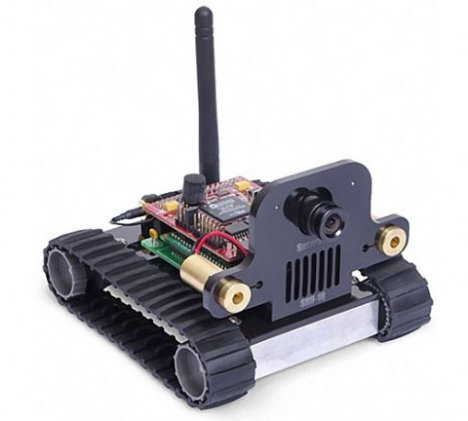
\includegraphics[scale=0.27]{srvq.jpg}
    \end{figure}
    SRV-1 Surveyor Robot
\end{columns}
\transboxout
\end{frame}

\begin{frame}\frametitle{States}
\begin{itemize}
\item[] For a robot whose current state is $x_k \in X$ at stage $k$,

\item[] we can update its state using a transition function $F(x_k, u_k)$ by applying its current action $u_k$.

\item[] Consider the moving uncertainty, we can describe the set of possible states at stage $k+1$
\end{itemize}
\begin{description}
\item
    \begin{figure}
    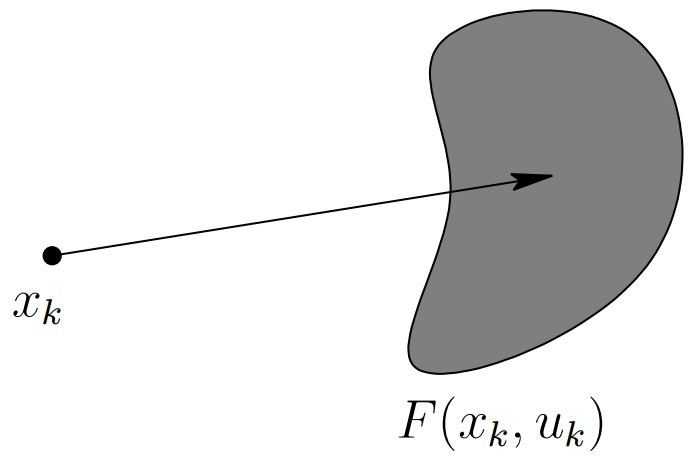
\includegraphics[scale=0.27]{istate.jpg}
    \end{figure}
\item Robot's state transition with uncertainty [\emph{Planning Algorithms}, S. LaValle, 2006]
\end{description}

\transboxin
\end{frame}

\begin{frame}\frametitle{Information States}
Assume that current real state of the robot could not be observed directly. \\

The robot could maintain a set of possible states, which is \emph{I-state} $\eta_k$,
 to make its decisions.
\begin{description}
\item
 \begin{figure}
    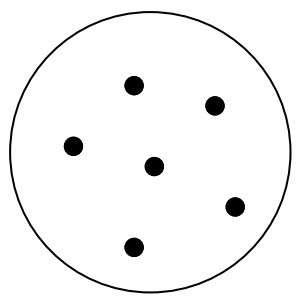
\includegraphics[scale=0.3]{xk.jpg}
    \end{figure}
 \item $\eta_k$ : contains all possible states at stage $k$ [\emph{Planning Algorithms}, S. LaValle, 2006]
 \end{description}
%
%
%\begin{itemize}
%\item A set-valued \emph{state transition function} $F: X \times U \to X$ \\
%    $F(x_k, u_k) = \left\{x_k + u_k + \theta_k \mid \theta_k \in \Theta(u_k)\right\} \cap X_{free}$\\
%    where $\Theta(u_k)$ denotes a bounded set of possible noise values, which
%	may depend on the action the robot selects.
%
%\item A set-valued \emph{observation function} $h: X \to Y$\\
%    $H(y_k) = \left\{ x_k \in X \mid y_k \in h(x_k), y_k \in Y \right\}$
%\end{itemize}

\transboxout
\end{frame}

\begin{frame}\frametitle{Set Transition Function}
Assume that current real state of the robot can not be observed directly. \\

The robot could maintain a set of possible states, which is \emph{I-state} $\eta_k$,
 to make its decisions.
\begin{description}
\item \begin{figure}
    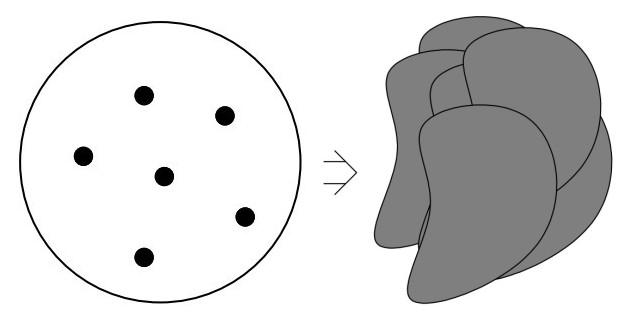
\includegraphics[scale=0.3]{xk_u.jpg}
    \end{figure}
\item For each $x_k \in \eta_k$, applying set-valued transition function $F$ yields $\bigcup_{x_k \in \eta_k} F(x_k, u_k)$.
    [\emph{Planning Algorithms}, S. LaValle, 2006]
\end{description}
\transboxout
\end{frame}

\begin{frame}\frametitle{Set Observation Function}
\begin{columns}
\column{.6\textwidth}
\begin{itemize}
\item Assume the observation preimage $H(y_k) \in X$ derived from the observation function $h: X \to Y$,
is a planar disk, where $y_k \in Y$ is the observation. \\

\item The \emph{I-state} could be updated by intersecting transited set of possible states with the
observation preimage:\\
\begin{equation}\label{eq:itrans}
		\eta_{k+1} =
		 \left[ \bigcup_{x_k \in \eta_k} F(x_k, u_k) \right]
		\cap H(y_k).
	\end{equation}
\end{itemize}
\column{.4\textwidth}
 \begin{figure}
    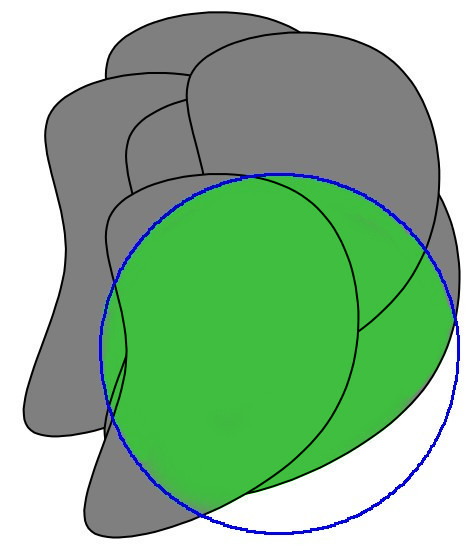
\includegraphics[scale=0.25]{xk_intersect.jpg}
    \caption{The green region is updated \emph{I-state} $\eta_{k+1}$}
    \end{figure}
\end{columns}
\transboxout
\end{frame}

\begin{frame}\frametitle{Prior Work}
\begin{itemize}
\item[] Prior research done by (B. Tovar and S. M. LaValle) and (J. van den Berg, P. Abbeel, and K. Goldberg)
used probabilistic representations for planning\\

\item[] Prior work by the authors (J.O'Kane) has used preliminary versions of the constrained geometric approximation method using specific, fixed range spaces. \\
\end{itemize}
New contributions
\begin{enumerate}
\item A careful formulation of the operations in the range space $\mathcal{R}$.
\item Algorithms for double-rectangle range space $\mathcal{R}_{drect}$.
\item A series of experiments for effectiveness comparison of different range spaces.
\end{enumerate}
\transboxin
\end{frame}

\begin{frame}
  \frametitle{Outlines}
  \tableofcontents[]
  \transboxout
\end{frame}
\section[Range Space]{Range Space}

\subsection[Range Space Definition]{Range Space Definition}
\begin{frame} \frametitle{Range Space}
\begin{definition}{\textbf{A range space}}
 $\mathcal{R} \subseteq \mathcal{I}$ is a set of I-states, contains
 approximation of \emph{I-states}, $A(\eta_k) \in \mathcal{R}$, equipped with
 two operations:
\end{definition}
\begin{columns}
\column{.6\textwidth}
\begin{enumerate}
\item An \emph{approximate observation update function} $O: \mathcal{R} \times
		Y \to \mathcal{R}$, such that if $\eta_k \subseteq A(\eta_k)$, then
			$$\eta_k \cap H(y_k) \subseteq O(A(\eta_k), u_k)$$
\item An \emph{approximate action update function} $T: \mathcal{R} \times U \to
		\mathcal{R}$, such that if $\eta_k \subseteq A(\eta_k)$, then
			$$\bigcup_{x_k \in \eta_k} F(x_k, u_k) \subseteq T(A(\eta_k), u_k)$$
\end{enumerate}
\column{.4\textwidth}
    \begin{figure}
    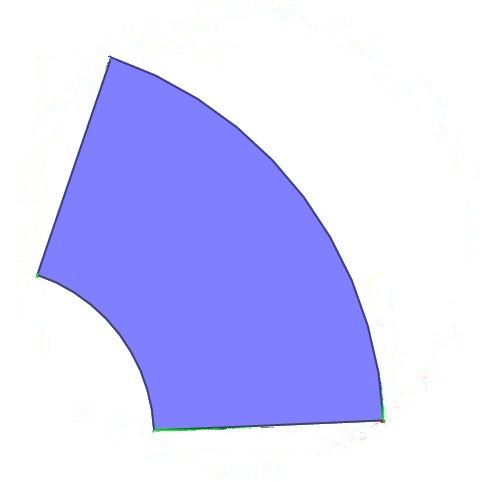
\includegraphics[scale=0.3]{norangespace.jpg}
    \caption{The blue region denotes the \emph{I-state} $\eta_k$}
    \end{figure}
\end{columns}
\end{frame}


\begin{frame} \frametitle{Range Space}
\begin{definition}{\textbf{A range space}}
 $\mathcal{R} \subseteq \mathcal{I}$ is a set of I-states, contains
 approximation of \emph{I-states}, $A(\eta_k) \in \mathcal{R}$, equipped with
 two operations:
\end{definition}
\begin{columns}
\column{.6\textwidth}
\begin{enumerate}
\item An \emph{approximate observation update function} $O: \mathcal{R} \times
		Y \to \mathcal{R}$, such that if $\eta_k \subseteq A(\eta_k)$, then
			$$\eta_k \cap H(y_k) \subseteq O(A(\eta_k), u_k)$$
\item An \emph{approximate action update function} $T: \mathcal{R} \times U \to
		\mathcal{R}$, such that if $\eta_k \subseteq A(\eta_k)$, then
			$$\bigcup_{x_k \in \eta_k} F(x_k, u_k) \subseteq T(A(\eta_k), u_k)$$
\end{enumerate}
\column{.4\textwidth}
    \begin{figure}
    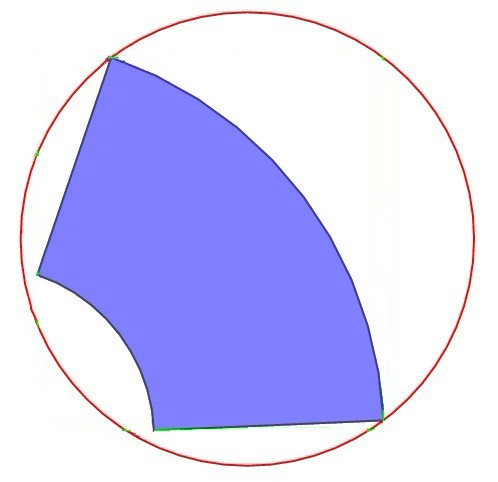
\includegraphics[scale=0.3]{rangespace_circle.jpg}
    \caption{Disk overapproximation $A(\eta_k) \in \mathcal{R}_{disk}$ in red.}
    \end{figure}
\end{columns}
\end{frame}

\begin{frame} \frametitle{Range Space}
\begin{definition}{\textbf{A range space}}
 $\mathcal{R} \subseteq \mathcal{I}$ is a set of I-states, contains
 approximation of \emph{I-states} $A(\eta_k) \in \mathcal{R}$, equipped with
 two operations:
\end{definition}
\begin{columns}
\column{.6\textwidth}
\begin{enumerate}
\item An \emph{approximate observation update function} $O: \mathcal{R} \times
		Y \to \mathcal{R}$, such that if $\eta_k \subseteq A(\eta_k)$, then
			$$\eta_k \cap H(y_k) \subseteq O(A(\eta_k), u_k)$$
\item An \emph{approximate action update function} $T: \mathcal{R} \times U \to
		\mathcal{R}$, such that if $\eta_k \subseteq A(\eta_k)$, then
			$$\bigcup_{x_k \in \eta_k} F(x_k, u_k) \subseteq T(A(\eta_k), u_k)$$
\end{enumerate}
\column{.4\textwidth}
    \begin{figure}
    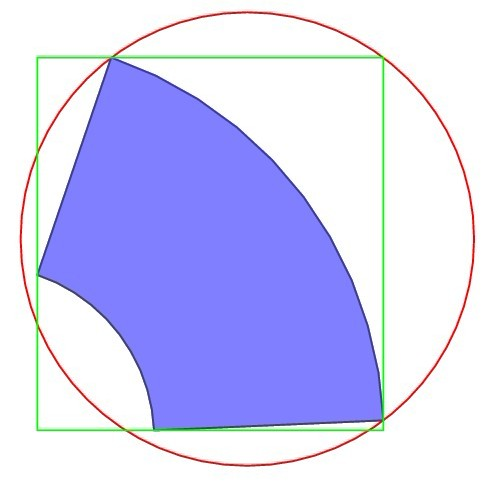
\includegraphics[scale=0.3]{rangespace.jpg}
    \caption{Rectangle overapproximation $A(\eta_k) \in \mathcal{R}_{rect}$.}
    \end{figure}
\end{columns}
\end{frame}

\subsection[Disk Range Space]{Disk Range Space}
\begin{frame} \frametitle{Observation Update in Disk Range Space $\mathcal{R}_{disk}$}
 Approximated I-state $A(\eta_k) \in \mathcal{R}_{disk}$, where $x_k$ denotes the real state but unknown to robot.
			
    \begin{figure}
    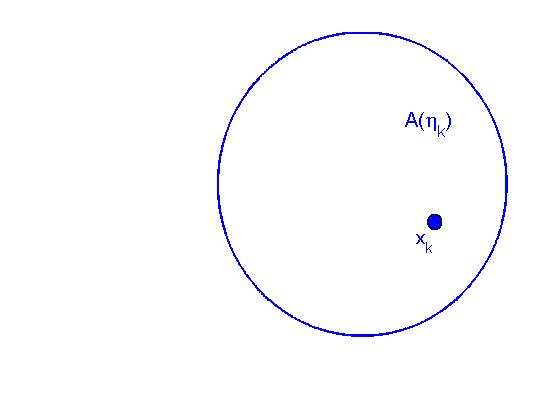
\includegraphics[scale=0.3]{circle1_2.jpg}
    \end{figure}
\transboxout
\end{frame}

\begin{frame} \frametitle{Observation Update in Disk Range Space $\mathcal{R}_{disk}$}
 Approximated I-state $A(\eta_k) \in \mathcal{R}_{disk}$ intersects with observation preimage $H(y_k)$ .
			
    \begin{figure}
    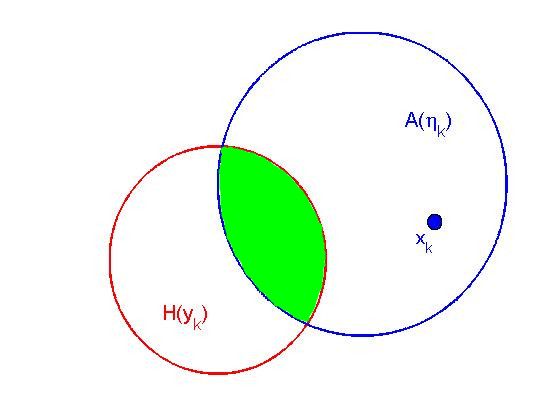
\includegraphics[scale=0.3]{circle2_2.jpg}
    \end{figure}
\transboxout		
\end{frame}

\begin{frame} \frametitle{Observation Update in Disk Range Space $\mathcal{R}_{disk}$}
 The green region of intersection is the updated I-state $\eta_{k+1}$, and the green disk
    is the approximation $A(\eta_{k+1})$ of $\eta_{k+1}$.
			
    \begin{figure}
    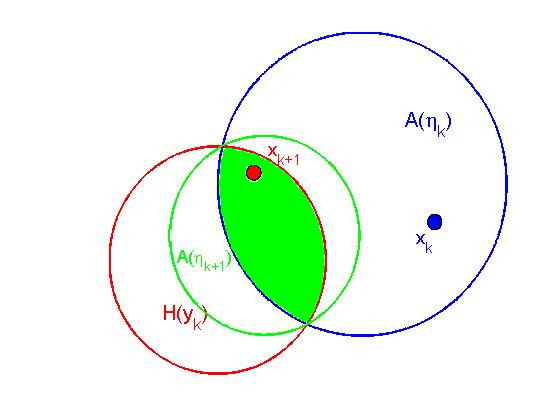
\includegraphics[scale=0.3]{circle3_2.jpg}
    \end{figure}
\transboxout
\end{frame}

\subsection[Rectangle Range Space]{Rectangle Range Space}
%%%%%%%%%%%%%%%%%%%%%%%%%%%%%%%%%%%%%%%%%%%%%%%%%%%%%%%%%%%%%%%%%%%%%%%%%%%%%%%%%%%%%%%%%%%%%%%%%%%%%%%%%
\begin{frame} \frametitle{Observation Update in $\mathcal{R}_{rect}$}
\begin{definition}{\textbf{$AABB(S)$} :}
    For any compact set $S \subset \mathbb{R}^2$, let $AABB(S)$
	denote the its smallest	``axis-aligned bounding box.''
\end{definition}

In $\mathcal{R}_{rect}$, computing approximate observation update function $O_{rect}$ takes $O(1)$ time:\\
$$ O_{rect}(A_k, y_k) = AABB(H(y_k) \cap A(\eta_k)), A_k = A(\eta_k) \in \mathcal{R}_{rect}$$

\begin{figure}
    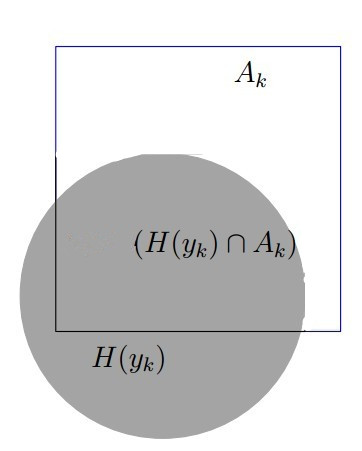
\includegraphics[scale=0.27]{circlerect_1.jpg}
    \end{figure}
\transboxout
\end{frame}


\begin{frame} \frametitle{Observation Update in $\mathcal{R}_{rect}$}
\begin{definition}{\textbf{$AABB(S)$} :}
    For any compact set $S \subset \mathbb{R}^2$, let $AABB(S)$
	denote the its smallest	``axis-aligned bounding box.''
\end{definition}

In $\mathcal{R}_{rect}$, computing approximate observation update function $O_{rect}$ takes $O(1)$ time:\\
$$ O_{rect}(A_k, y_k) = AABB(H(y_k) \cap A(\eta_k)), A_k = A(\eta_k) \in \mathcal{R}_{rect}$$
    \begin{figure}
    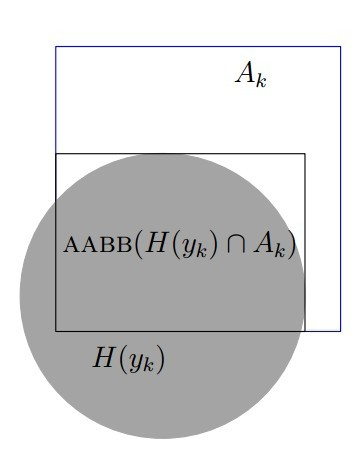
\includegraphics[scale=0.27]{circlerect.jpg}
    \end{figure}
\transboxout
\end{frame}
%%%%%%%%%%%%%%%%%%%%%%%%%%%%%%%%%%%%%%%%%%%%%%%%%%%%%%%%%%%%%%%%%%%%%%%%%%%%%%%%%%%%%%%%%%%%%%%%%%%%%%%

\begin{frame} \frametitle{Action Update in $\mathcal{R}_{rect}$}
In $\mathcal{R}_{rect}$, computing approximate action update function $T_{rect} :$\\
			$$T_{rect}(A(\eta_k), u_k) = AABB(X_{free} \cap [A(\eta_k) \oplus \{ u_k \} \oplus AABB(\Theta(u_k))])$$
    \begin{figure}
    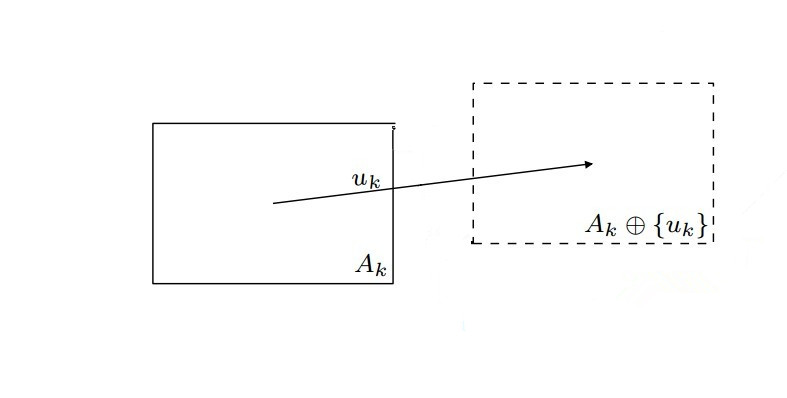
\includegraphics[scale=0.35]{t_rect.jpg}
    \caption{Transition of $A(\eta_k)$ given action $u_k$, $\oplus$ is Minkowski addition of two sets.}
    \end{figure}
\transboxout
\end{frame}

\begin{frame} \frametitle{Action Update in $\mathcal{R}_{rect}$}
In $\mathcal{R}_{rect}$, computing approximate action update function $T_{rect} :$\\
			$$T_{rect}(A(\eta_k), u_k) = AABB(X_{free} \cap [A(\eta_k) \oplus \{ u_k \} \oplus AABB(\Theta(u_k))])$$
    \begin{figure}
    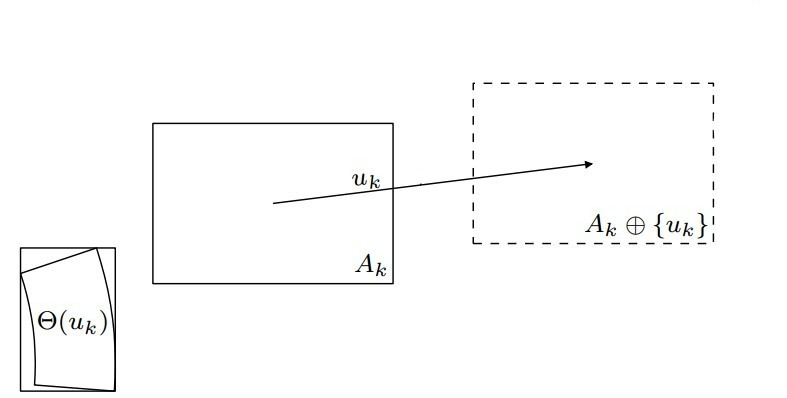
\includegraphics[scale=0.35]{t_rect2.jpg}
    \caption{Consider approximation of the bounded motion uncertainty $\Theta(u_k)$.}
    \end{figure}

\transboxout
\end{frame}

\begin{frame} \frametitle{Action Update in $\mathcal{R}_{rect}$}
In $\mathcal{R}_{rect}$, computing approximate action update function $T_{rect} :$\\
			$$T_{rect}(A(\eta_k), u_k) = AABB(X_{free} \cap [A(\eta_k) \oplus \{ u_k \} \oplus AABB(\Theta(u_k))])$$
    \begin{figure}
    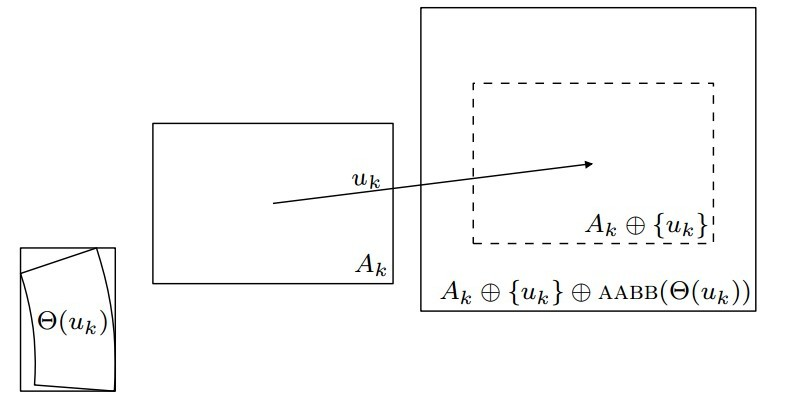
\includegraphics[scale=0.35]{step12.jpg}
    \caption{Find Minkowski sum of bounded noise and approximation transition}
    \end{figure}
		
\transboxout
\end{frame}


\begin{frame} \frametitle{Action Update in $\mathcal{R}_{rect}$}
In $\mathcal{R}_{rect}$, computing approximate action update function $T_{rect} :$\\
			$$T_{rect}(A(\eta_k), u_k) = AABB(X_{free} \cap [A(\eta_k) \oplus \{ u_k \} \oplus AABB(\Theta(u_k))])$$
    \begin{figure}
    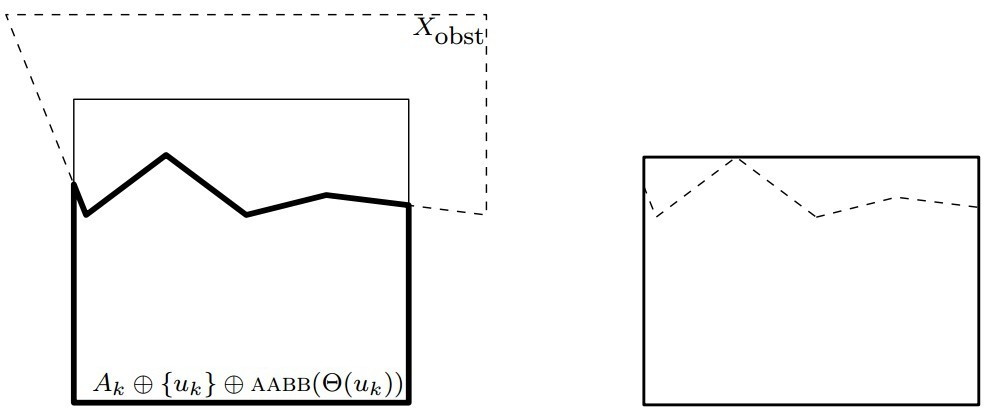
\includegraphics[scale=0.35]{step34.jpg}
    \caption{If there is obstacles, intersect with $X_{free}$ first and
    then find the bounding box of the intersection.}
    \end{figure}
		
\transboxout
\end{frame}

\begin{frame}
  \frametitle{Outlines}
  \tableofcontents[]
  \transboxout
\end{frame}
\section[Double-Rectangle Range Space]{Double-Rectangle Range Space}

\begin{frame}\frametitle{Double-Rectangle approximated I-state}
\begin{itemize}
\item  For better overapproximation quality for non-convex \emph{I-states},
we proposed a more expressive range space of \emph{double rectangles}: \\
\begin{equation}
	\mathcal{R}_{drect} = \{ R_1 \cup R_2 \mid R_1, R_2 \in \mathcal{R}_{rect} \}
\end{equation}
 \item Aims to improve the approximation quality.
\begin{figure}
    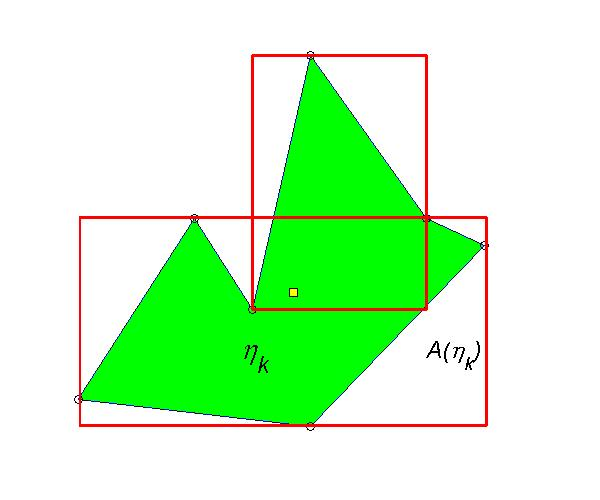
\includegraphics[scale=0.26]{poly.jpg}
    \caption{Non-convex \emph{I-state}}
 \end{figure}

\end{itemize}
\transboxin
\end{frame}
%%%%%%%%%%%%%%%%%%%%%%%%%%%%%%%%%%%%%%%%%%%%%%%%%%%%%%%%%%%%%%%%%%%%%%%%%%%%

\begin{frame} \frametitle{DRAP Algorithm}
``Double Rectangle Around Polygon'' (\textbf{DRAP}) algorithm:\\
\begin{itemize}
    \item input is a $n$-edge polygonal region of the plane
    \item output is a small double rectangle containing that polygon
    \item run time: $O(n^3)$
\end{itemize}

    \begin{figure}
    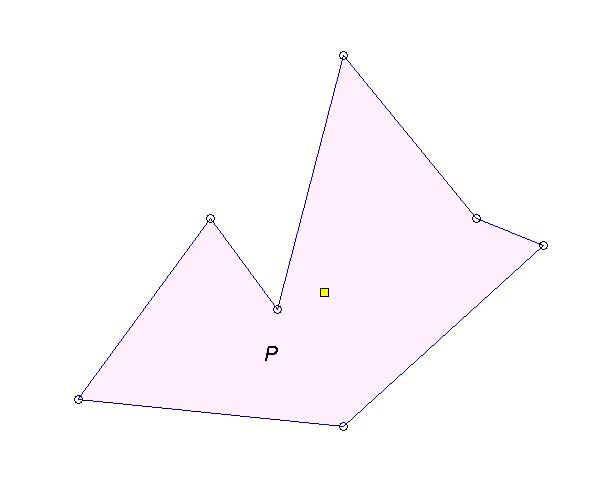
\includegraphics[scale=0.3]{drapP.jpg}
    \end{figure}

\transboxout
\end{frame}

\begin{frame} \frametitle{DRAP Algorithm}
``Double Rectangle Around Polygon'' (\textbf{DRAP}) algorithm:\\
\begin{itemize}
     \item input is a $n$-edge polygonal region of the plane
    \item output is a small double rectangle containing that polygon
    \item run time: $O(n^3)$
\end{itemize}

    \begin{figure}
    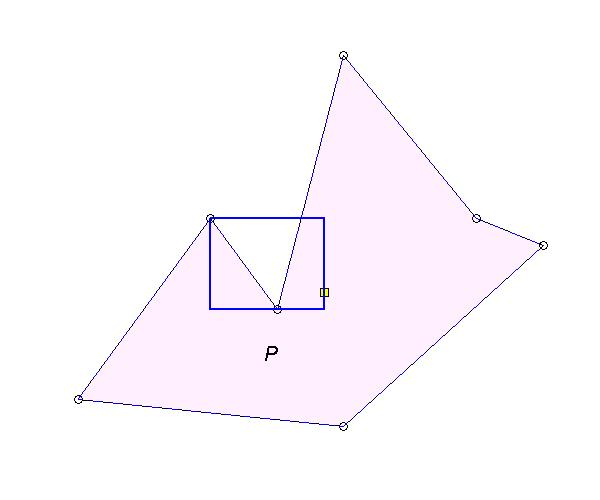
\includegraphics[scale=0.3]{drap1.jpg}
    \end{figure}

\transboxout
\end{frame}

\begin{frame} \frametitle{DRAP Algorithm}
``Double Rectangle Around Polygon'' (\textbf{DRAP}) algorithm:\\
\begin{itemize}
     \item input is a $n$-edge polygonal region of the plane
    \item output is a small double rectangle containing that polygon
    \item run time: $O(n^3)$
\end{itemize}

    \begin{figure}
    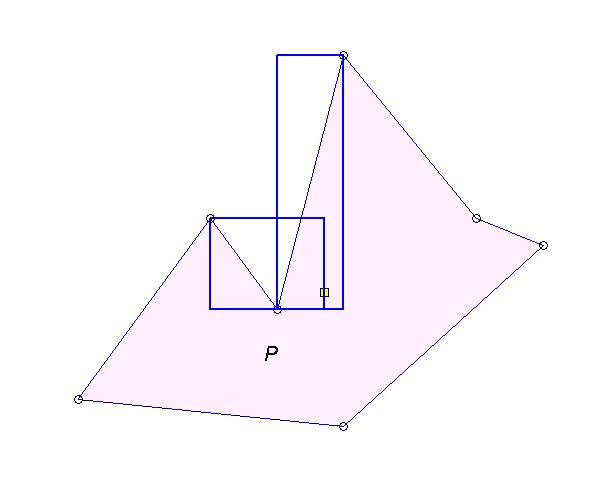
\includegraphics[scale=0.3]{drap2.jpg}
    \end{figure}


\transboxout
\end{frame}


\begin{frame} \frametitle{DRAP Algorithm}
``Double Rectangle Around Polygon'' (\textbf{DRAP}) algorithm:\\
\begin{itemize}
     \item input is a $n$-edge polygonal region of the plane
    \item output is a small double rectangle containing that polygon
    \item run time: $O(n^3)$
\end{itemize}

    \begin{figure}
    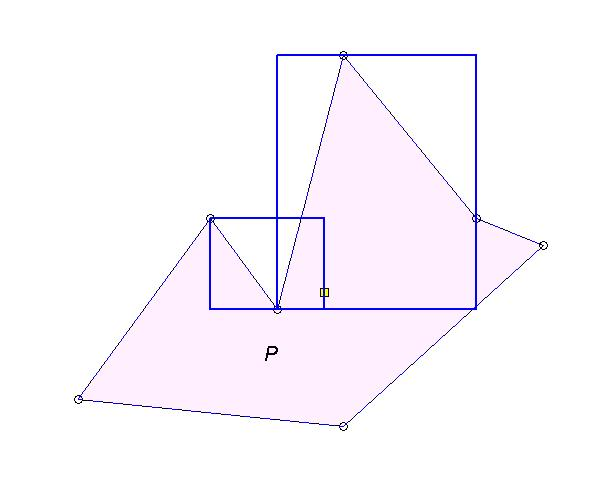
\includegraphics[scale=0.3]{drap3.jpg}
    \end{figure}

\transboxout
\end{frame}

\begin{frame} \frametitle{DRAP Algorithm}
``Double Rectangle Around Polygon'' (\textbf{DRAP}) algorithm:\\
\begin{itemize}
     \item input is a $n$-edge polygonal region of the plane
    \item output is a small double rectangle containing that polygon
    \item run time: $O(n^3)$
\end{itemize}

    \begin{figure}
    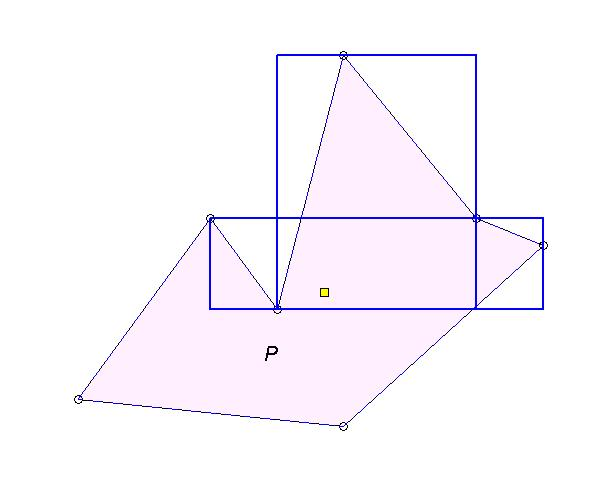
\includegraphics[scale=0.3]{drap4.jpg}
    \end{figure}


\transboxout
\end{frame}

\begin{frame} \frametitle{DRAP Algorithm}
``Double Rectangle Around Polygon'' (\textbf{DRAP}) algorithm:\\
\begin{itemize}
     \item input is a $n$-edge polygonal region of the plane
    \item output is a small double rectangle containing that polygon
    \item run time: $O(n^3)$
\end{itemize}

    \begin{figure}
    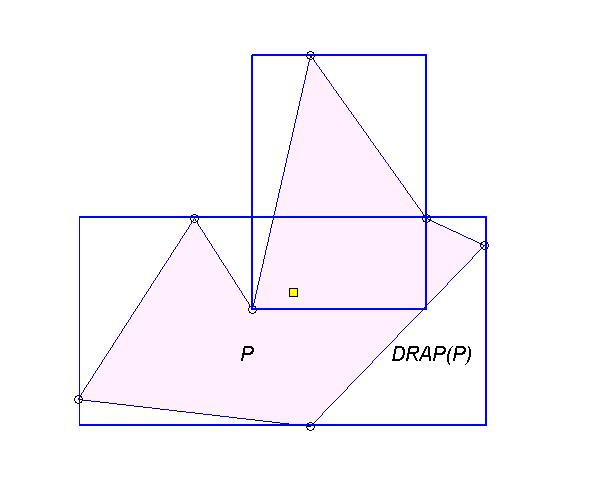
\includegraphics[scale=0.3]{drap.jpg}
    \end{figure}
\transboxout
\end{frame}
%%%%%%%%%%%%%%%%%%%%%%%%%%%%%%%%%%%%%%%%%%%%%%%%%%%%%%%%%%%%%%%%%%%%%%%%%%%%%%%%%%%%
\begin{frame} \frametitle{Operations in $\mathcal{R}_{drect}$}

Based on \textbf{DRAP} Algorithm, we can define the range space operations on
$\mathcal{R}_{drect}$ in a manner similar to those for $\mathcal{R}_{rect}$.  For a double rectangle
approximated \emph{I-state} $A(\eta_k) = R_1 \cup R_2$, we have
\begin{equation}
	T_{drect}(A(\eta_k), u_k) = DRAP(X_{free} \cap [A(\eta_k) \oplus \{ u_k \} \oplus DRAP(\Theta(u_k))]),
\end{equation}
\begin{equation}
	O_{drect}(A(\eta_k), y_k) = AABB(H(y_k) \cap R_1)\cup AABB(H(y_k) \cap R_2).
\end{equation}
\begin{figure}
    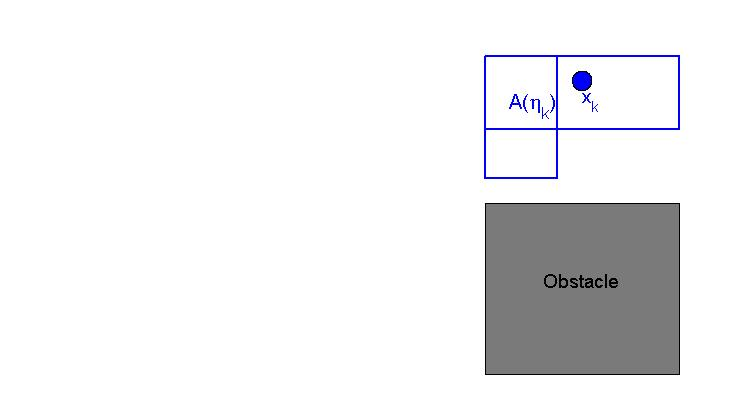
\includegraphics[scale=0.3]{drectevolve0.jpg}
    \end{figure}
\transboxout
\end{frame}

\begin{frame} \frametitle{Operations in $\mathcal{R}_{drect}$}

Based on \textbf{DRAP} Algorithm, we can define the range space operations on
$\mathcal{R}_{drect}$ in a manner similar to those for $\mathcal{R}_{rect}$.  For a double rectangle
approximated \emph{I-state} $A(\eta_k) = R_1 \cup R_2$, we have
\begin{equation}
	T_{drect}(A(\eta_k), u_k) = DRAP(X_{free} \cap [A(\eta_k) \oplus \{ u_k \} \oplus DRAP(\Theta(u_k))]),
\end{equation}
\begin{equation}
	O_{drect}(A(\eta_k), y_k) = AABB(H(y_k) \cap R_1)\cup AABB(H(y_k) \cap R_2).
\end{equation}
\begin{figure}
    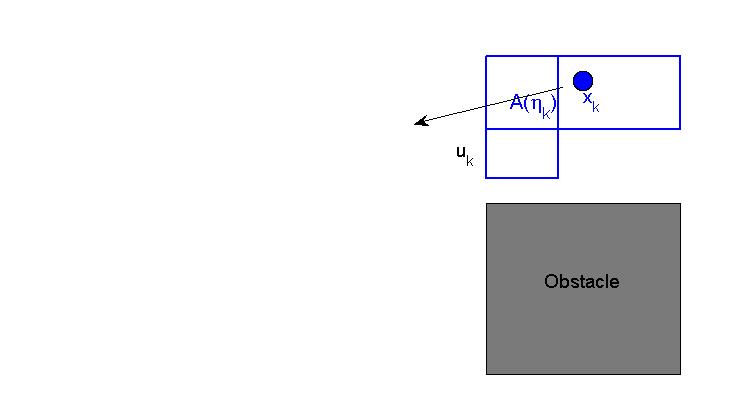
\includegraphics[scale=0.3]{drectevolve1.jpg}
    \end{figure}
\transboxout
\end{frame}

\begin{frame} \frametitle{Operations in $\mathcal{R}_{drect}$}

Based on \textbf{DRAP} Algorithm, we can define the range space operations on
$\mathcal{R}_{drect}$ in a manner similar to those for $\mathcal{R}_{rect}$.  For a double rectangle
approximated \emph{I-state} $A(\eta_k) = R_1 \cup R_2$, we have
\begin{equation}
	T_{drect}(A(\eta_k), u_k) = DRAP(X_{free} \cap [A(\eta_k) \oplus \{ u_k \} \oplus DRAP(\Theta(u_k))]),
\end{equation}
\begin{equation}
	O_{drect}(A(\eta_k), y_k) = AABB(H(y_k) \cap R_1)\cup AABB(H(y_k) \cap R_2).
\end{equation}
\begin{figure}
    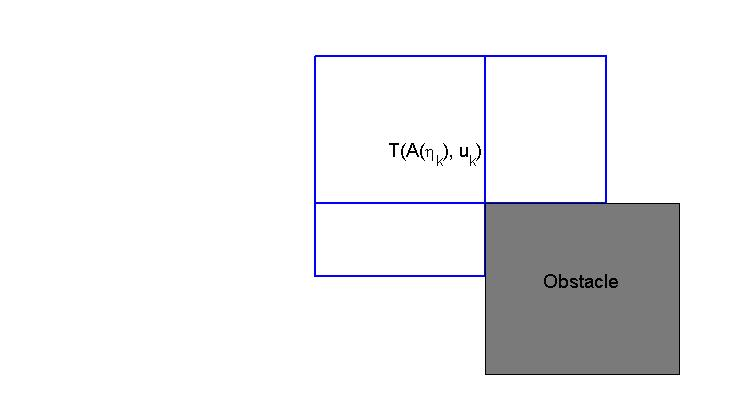
\includegraphics[scale=0.3]{drectevolve2.jpg}
    \end{figure}
\transboxout
\end{frame}

\begin{frame} \frametitle{Operations in $\mathcal{R}_{drect}$}

Based on \textbf{DRAP} Algorithm, we can define the range space operations on
$\mathcal{R}_{drect}$ in a manner similar to those for $\mathcal{R}_{rect}$.  For a double rectangle
approximated \emph{I-state} $A(\eta_k) = R_1 \cup R_2$, we have
\begin{equation}
	T_{drect}(A(\eta_k), u_k) = DRAP(X_{free} \cap [A(\eta_k) \oplus \{ u_k \} \oplus DRAP(\Theta(u_k))]),
\end{equation}
\begin{equation}
	O_{drect}(A(\eta_k), y_k) = AABB(H(y_k) \cap R_1)\cup AABB(H(y_k) \cap R_2).
\end{equation}
\begin{figure}
    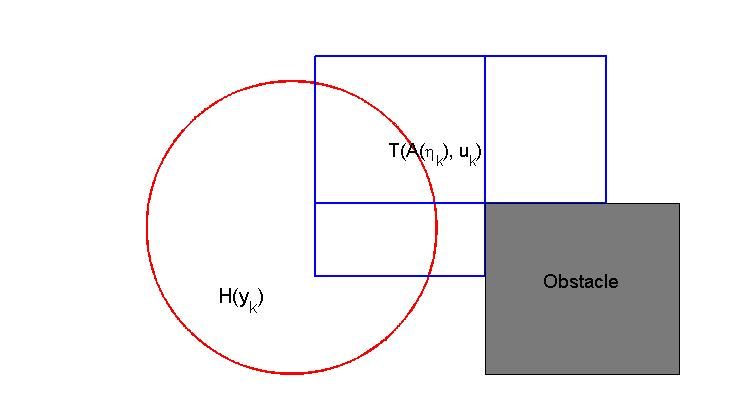
\includegraphics[scale=0.3]{drectevolve3.jpg}
    \end{figure}
\transboxout
\end{frame}

\begin{frame} \frametitle{Operations in $\mathcal{R}_{drect}$}

Based on \textbf{DRAP} Algorithm, we can define the range space operations on
$\mathcal{R}_{drect}$ in a manner similar to those for $\mathcal{R}_{rect}$.  For a double rectangle
approximated \emph{I-state} $A(\eta_k) = R_1 \cup R_2$, we have
\begin{equation}
	T_{drect}(A(\eta_k), u_k) = DRAP(X_{free} \cap [A(\eta_k) \oplus \{ u_k \} \oplus DRAP(\Theta(u_k))]),
\end{equation}
\begin{equation}
	O_{drect}(A(\eta_k), y_k) = AABB(H(y_k) \cap R_1)\cup AABB(H(y_k) \cap R_2).
\end{equation}
\begin{figure}
    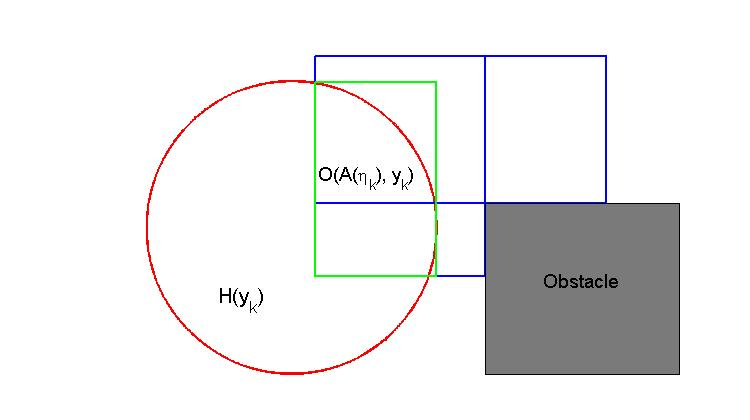
\includegraphics[scale=0.3]{drectevolve4.jpg}
    \end{figure}
\transboxout
\end{frame}

\begin{frame} \frametitle{Operations in $\mathcal{R}_{drect}$}

Based on \textbf{DRAP} Algorithm, we can define the range space operations on
$\mathcal{R}_{drect}$ in a manner similar to those for $\mathcal{R}_{rect}$.  For a double rectangle
approximated \emph{I-state} $A(\eta_k) = R_1 \cup R_2$, we have
\begin{equation}
	T_{drect}(A(\eta_k), u_k) = DRAP(X_{free} \cap [A(\eta_k) \oplus \{ u_k \} \oplus DRAP(\Theta(u_k))]),
\end{equation}
\begin{equation}
	O_{drect}(A(\eta_k), y_k) = AABB(H(y_k) \cap R_1)\cup AABB(H(y_k) \cap R_2).
\end{equation}
\begin{figure}
    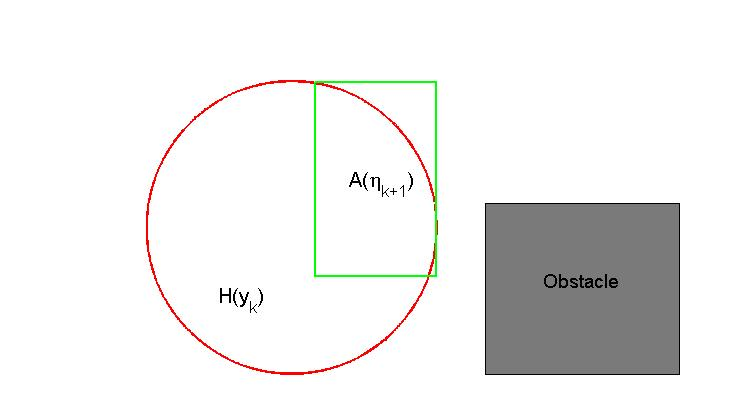
\includegraphics[scale=0.3]{drectevolve5.jpg}
    \end{figure}
\transboxout
\end{frame}

%%%%%%%%%%%%%%%%%%%%%%%%%%%%%%%%%%%%%%%%%%%%%%%%%%%%%%%%%%%%%%%%%%%%%%%%%%%%%%%%%%%%
\begin{frame}
  \frametitle{Outlines}
  \tableofcontents[]
  \transboxout
\end{frame}
\section[Experiments]{Experiments}

\begin{frame}\frametitle{Experiments: Task in Various Environments}
To verify the effectiveness and efficiency of CGA for a navigation task,
in comparison with using the true \emph{information state},
we conducted experiments using 3 environments, and 3 range spaces $\mathcal{R}_{disk}$, $\mathcal{R}_{rect}$, and
$\mathcal{R}_{drect}$. \\

\textbf{ASSUMPTIONS:}\\
\begin{itemize}
\item A point robot follows predefined waypoints guided by centroid point of the approximated \emph{I-state}
\item Robot can detect presence but not distance to the waypoints
\item Landmarks are pseudo-randomly generated (Number Matters)
\item Initial I-state $\eta_0$ is given.
\end{itemize}

\movie[externalviewer]{\beamergotobutton{Start movie}}{clutter_dbrect.avi}
\end{frame}


\begin{frame}\frametitle{Experiments Results}
For each environment, we measure:\\
\begin{itemize}
	\item the relationship between task completion and number of landmarks,
	\item the time required to compute approximated \emph{I-state} compared to the
	       high-quality polygonal representation of the exact \emph{I-state},
	\item the approximation ratio $Q_k$\\
        \begin{equation}
	       Q_k = \frac{1}{k} \sum_{i=1}^k \frac{\mathbb{A}(\eta_i)}{\mathbb{A}(A(\eta_i))}
        \end{equation}
        where $\mathbb{A}(\diamond)$ denotes the area of set $\diamond \subset \mathbb{R}^2$
\end{itemize}
\transboxout
\end{frame}


\begin{frame}\frametitle{Comparison of Efficiency and Accuracy}
\begin{columns}
\column{.5\textwidth}
    \begin{figure}
    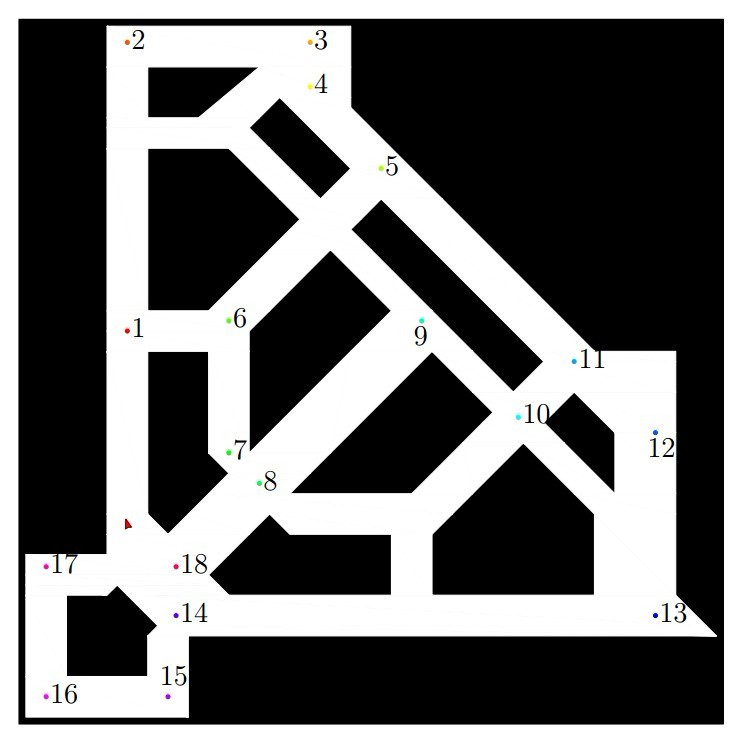
\includegraphics[scale=0.3]{office.jpg}
    \end{figure}
\column{.5\textwidth}
Comparison of the computation time and approximation ratio for approximated I-states
    to the corresponding computation for the exact \emph{I-states} shows
    the trade-off between time and accuracy.

    \begin{figure}
    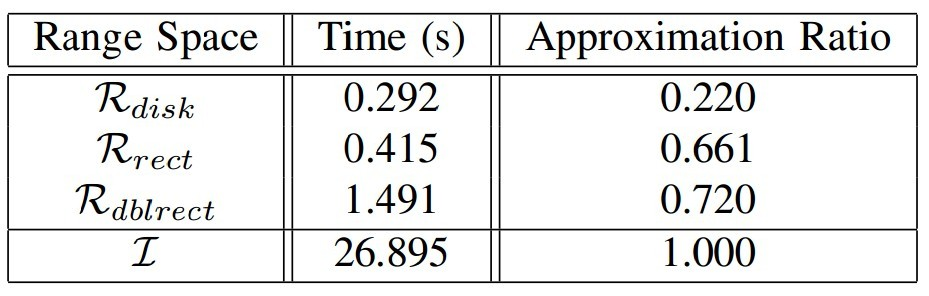
\includegraphics[scale=0.25]{tab1.jpg}
    \end{figure}


\end{columns}
\end{frame}

\begin{frame} \frametitle{Comparison of Success Rate in Office-like Environment}
\begin{figure}
    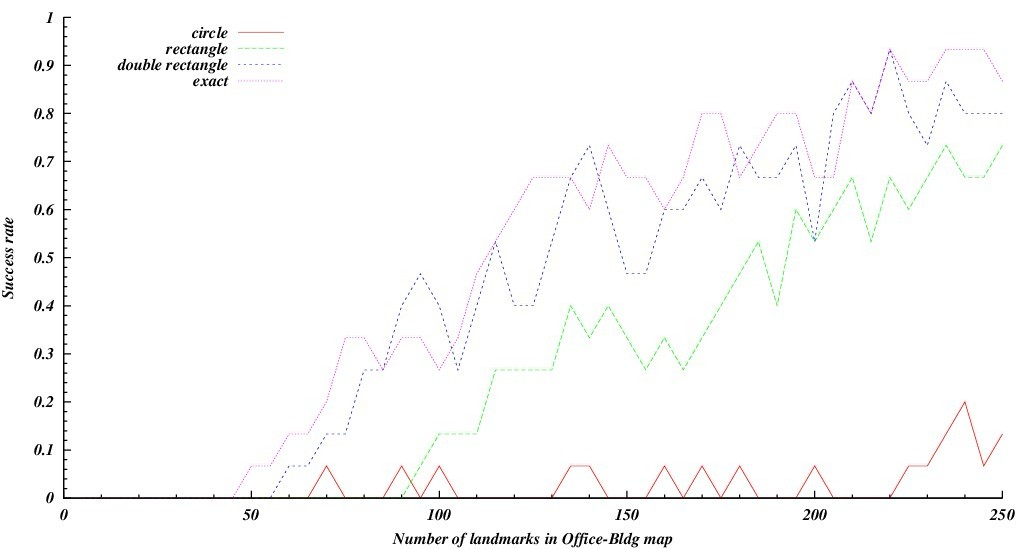
\includegraphics[scale=0.44]{rate-office.jpg}
    %\caption{For an environment with complex obstacles, $\mathcal{R}_{dblrest}$ shows
    %better performance than using $\mathcal{R}_{disk}$ or $\mathcal{R}_{rect}$ and
    %achieve almost same success rate compared to the true I-states.}
\end{figure}
\end{frame}

\begin{frame} \frametitle{Computation and Approximation ratio in Obstacle-free Environment}
\begin{figure}
    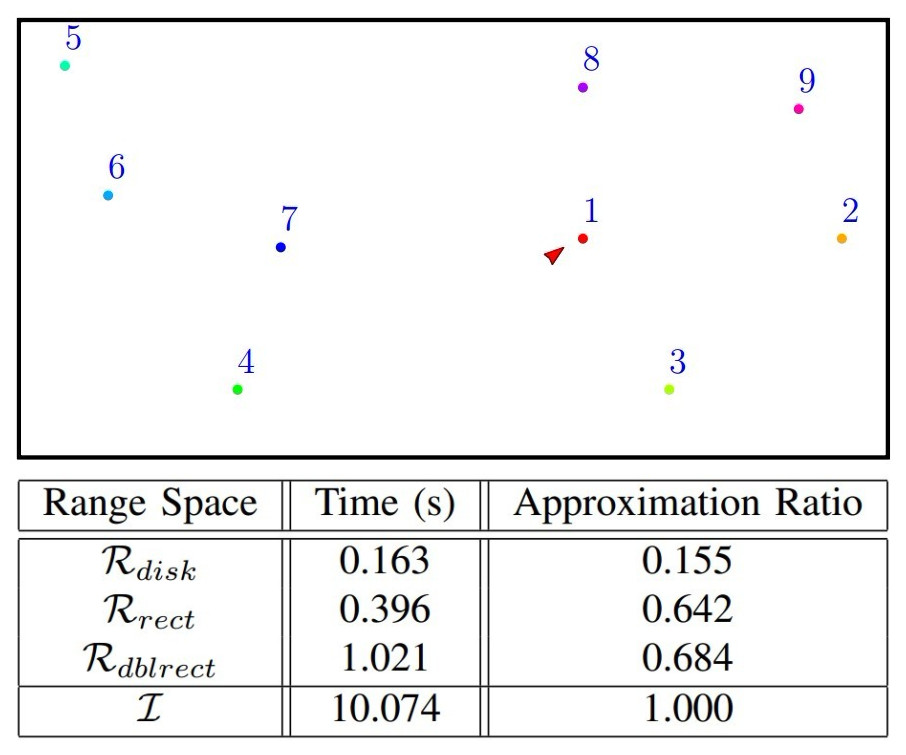
\includegraphics[scale=0.35]{obs_tab.jpg}
    %\caption{For an environment with complex obstacles, $\mathcal{R}_{dblrest}$ shows
    %better performance than using $\mathcal{R}_{disk}$ or $\mathcal{R}_{rect}$ and
    %achieve almost same success rate compared to the true I-states.}
\end{figure}
\end{frame}

\begin{frame} \frametitle{Comparison of Success Rate in Obstacle-free Environment}

\begin{figure}
    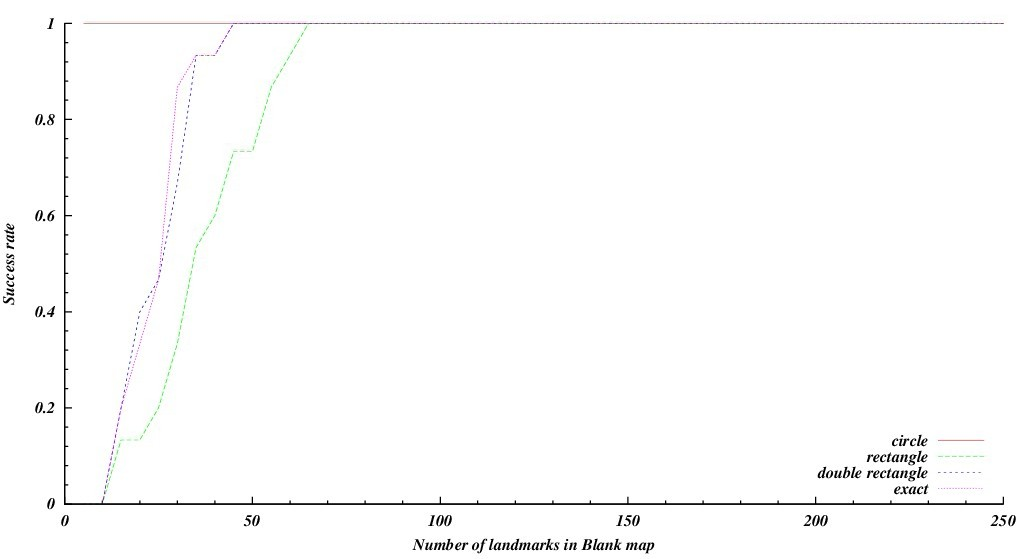
\includegraphics[scale=0.44]{rate-obs.jpg}
    %\caption{The success rate is related with the number of landmarks.
    %In the obstacle-free environment, the success rates for a robot to complete the task are
    %nearly identical using $\mathcal{R}_{disk}$, $\mathcal{R}_{rect}$, $\mathcal{R}_{dblrest}$ and true
    %I-states.}
\end{figure}
\end{frame}

\begin{frame} \frametitle{Computation and Approximation ratio in Obstacle-clutter Environment}
\begin{figure}
    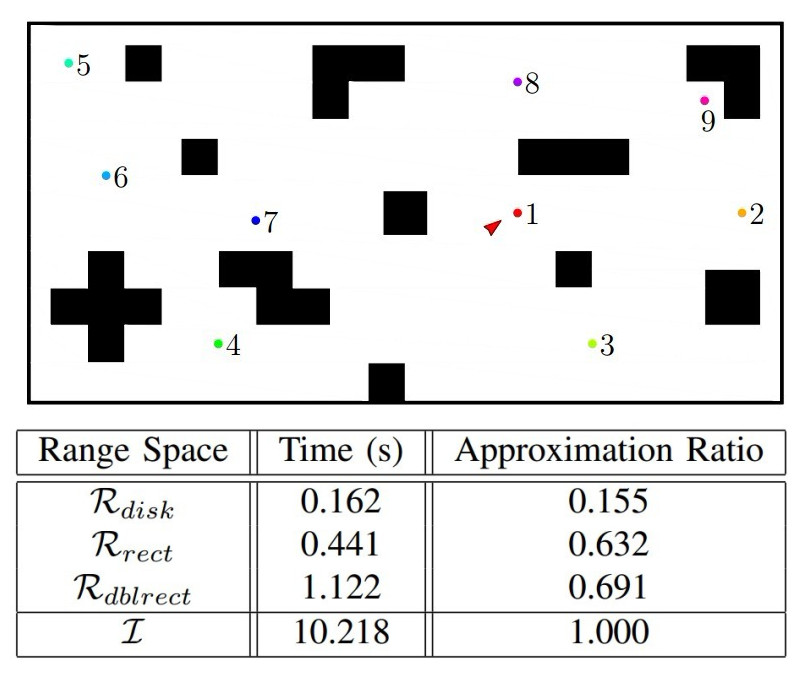
\includegraphics[scale=0.4]{clutter_tab.jpg}
    %\caption{For an environment with complex obstacles, $\mathcal{R}_{dblrest}$ shows
    %better performance than using $\mathcal{R}_{disk}$ or $\mathcal{R}_{rect}$ and
    %achieve almost same success rate compared to the true I-states.}
\end{figure}
\end{frame}

\begin{frame} \frametitle{Comparison of Success Rate in Obstacle-clutter Environment}
\begin{figure}
    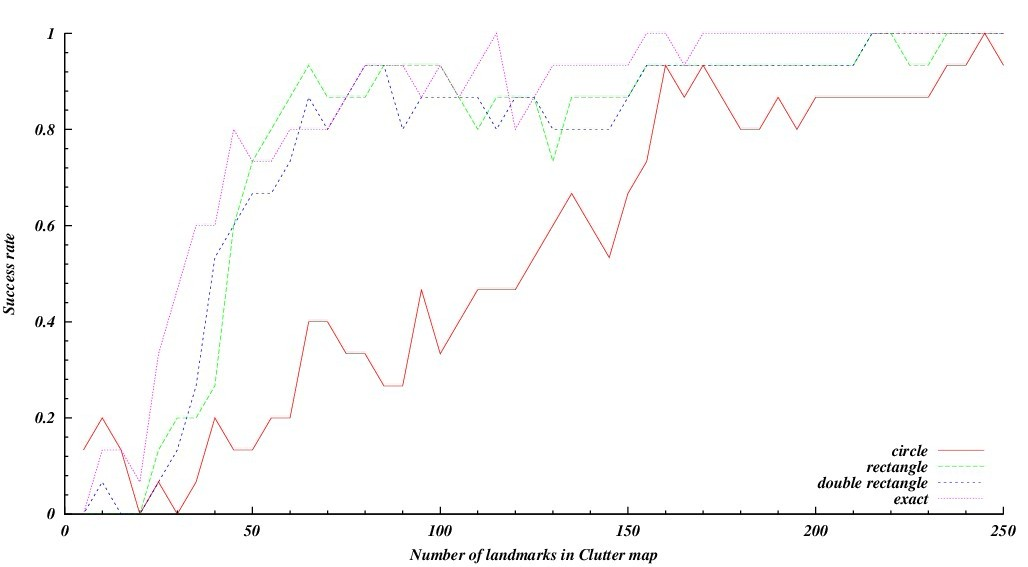
\includegraphics[scale=0.44]{rate-clutter.jpg}
    %\caption{Using $\mathcal{R}_{rect}$, $\mathcal{R}_{dblrest}$, achieve similar
    %performance to the true	I-state. Using $\mathcal{R}_{disk}$ yields lower success
    %rate due to the high possibility of collisions.}
\end{figure}
\end{frame}


\begin{frame}
  \frametitle{Outlines}
  \tableofcontents[]
  \transboxout
\end{frame}
\section[Conclusions]{Conclusions}
\begin{frame} \frametitle{Conclusions and Future Work}
\begin{itemize}
\item \textbf{\textcolor[rgb]{0.50,0.00,0.00}{Conclusions:}}
    \begin{enumerate}
    \item Constrained geometric approximation is effective for representing a robot's
    uncertain information about the current state.
    \item The form of double-rectangle is more accurate in approximating the non-convex
    \emph{I-state}.
    \item The robot can complete the navigation task using approximated I-state with
    low approximation accuracy.
    \end{enumerate}
\item \textbf{\textcolor[rgb]{0.50,0.00,0.00}{Future Work:}}
    \begin{enumerate}
    \item Additional range spaces, such as $k$-fold union of rectangles,
     will be considered to be used for high-accuracy approximation.

    \item There may also be some advantage to
    algorithms that also generate provable \textbf{under-approximates} of the I-state.
    \end{enumerate}
\end{itemize}
\transboxout
\end{frame}

\begin{frame} \frametitle{}
\begin{columns}
\column{.7\textwidth}
\begin{figure}
    
\includegraphics[scale=0.22]{scarr-logo.jpg}
\end{figure}
\column{.3\textwidth}
\begin{figure}
    \includegraphics[scale=0.4]{NSF_logo.jpg}
\end{figure}
\end{columns}
\begin{center}
\begin{figure}
    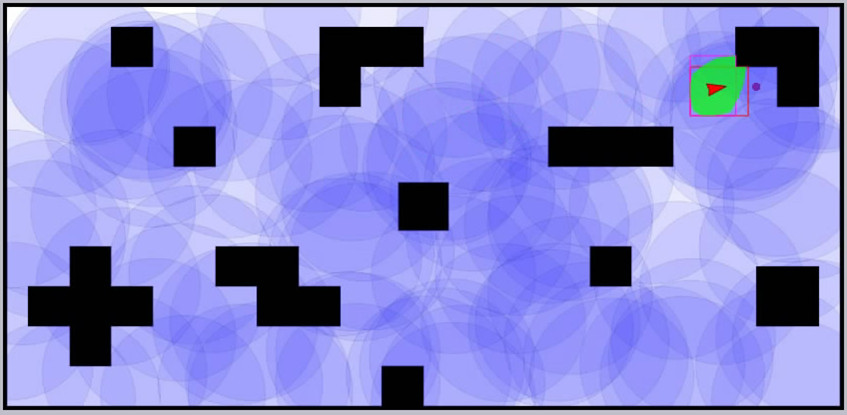
\includegraphics[scale=0.25]{clutter_dbrect_cover.jpg}
\end{figure}
\textcolor[rgb]{0.50,0.00,0.00}{\textbf{song24@email.sc.edu}}
\end{center}

\transboxout
\end{frame}


\end{document}
